\chapter{Exploration of atomistic predictions}
\label{chapter2}

Atomic interactions are a cornerstone of developing chemical 

However, this raises a vital question to the efficacy of ML models: how do we assess the reliability of ANI models for systems that exceed the size limitations of QM computations?

Accuracy is well-defined in quantum chemical methods via systematic convergence and comparison to experimental data, but approximating the results of QM computations with machine learning it is difficult to measure accuracy 

The ANAKIN-ME methodology provides a framework for atom-wise decomposition of molecular energies by using the atomic environment vector (AEV) representation to encode localized chemical interactions.

\section{ANAKIN-ME predictions}
\label{sec:ANI_predictions}

A decomposition approach allows for efficient, scalable predictions of energy for systems larger than the training data represents.
This is advantageous for simulating large systems, due to the size limitations of \textit{ab initio} computations.

To explore the trends in atomic energy predictions, a small testing subset was created using the first conformer of each molecular formula in the training dataset.
This testing set, referred to as 1x-test, will be used to explore some trends in atomic energies.

Here I should be writing about the ANI predictions in greater detail than the background information

Add content from pages 5-15 of qualifying exam document -- will need significant rewriting, but the details of the work completed there is useful for filling this section in. 


\subsection{Total energy as a sum of atomic energies}
\label{subsec:total_E_sum_AEs}

Though some partitioning schemes exist in quantum theory, such as Bader's Atoms in Molecules \cite{bader_aim}, there is no general consensus for decomposing the energy of a molecular system into a sum of atomic contributions.
The 

Eqn. \ref{eq:total_E_sum_AEs}, where $E_{\text{Total}}$ is the molecular energy prediction, $\varepsilon_i$ is the atomic energy contribution for atom $i$, and $\text{GSAE}_i$ is the ground state atomic energy for atom $i$.
The ground state atomic energies for each atom in the ANI networks are given in \ref{appendix:GSAEs}.

\begin{equation}
    E_{\text{Total}} = \sum_{i}^{\text{atoms}} \varepsilon_i + \text{GSAE}_i
    \label{eq:total_E_sum_AEs}
\end{equation}

\authorRemark{Here you should compare 2x atomic energy predictions to the 2xr predicitons, discuss how the distributions are shifted due to retraining with GSAEs but also note that the distributions are shaped differently, and models do not agree on what atomic energy partition should be.
Mention that with GSAEs we train networks without biases -- such that they learn to predict atomic energies as deviations from their isolated, ground state atomic energies.}

\begin{figure}[!ht]
    \centering
    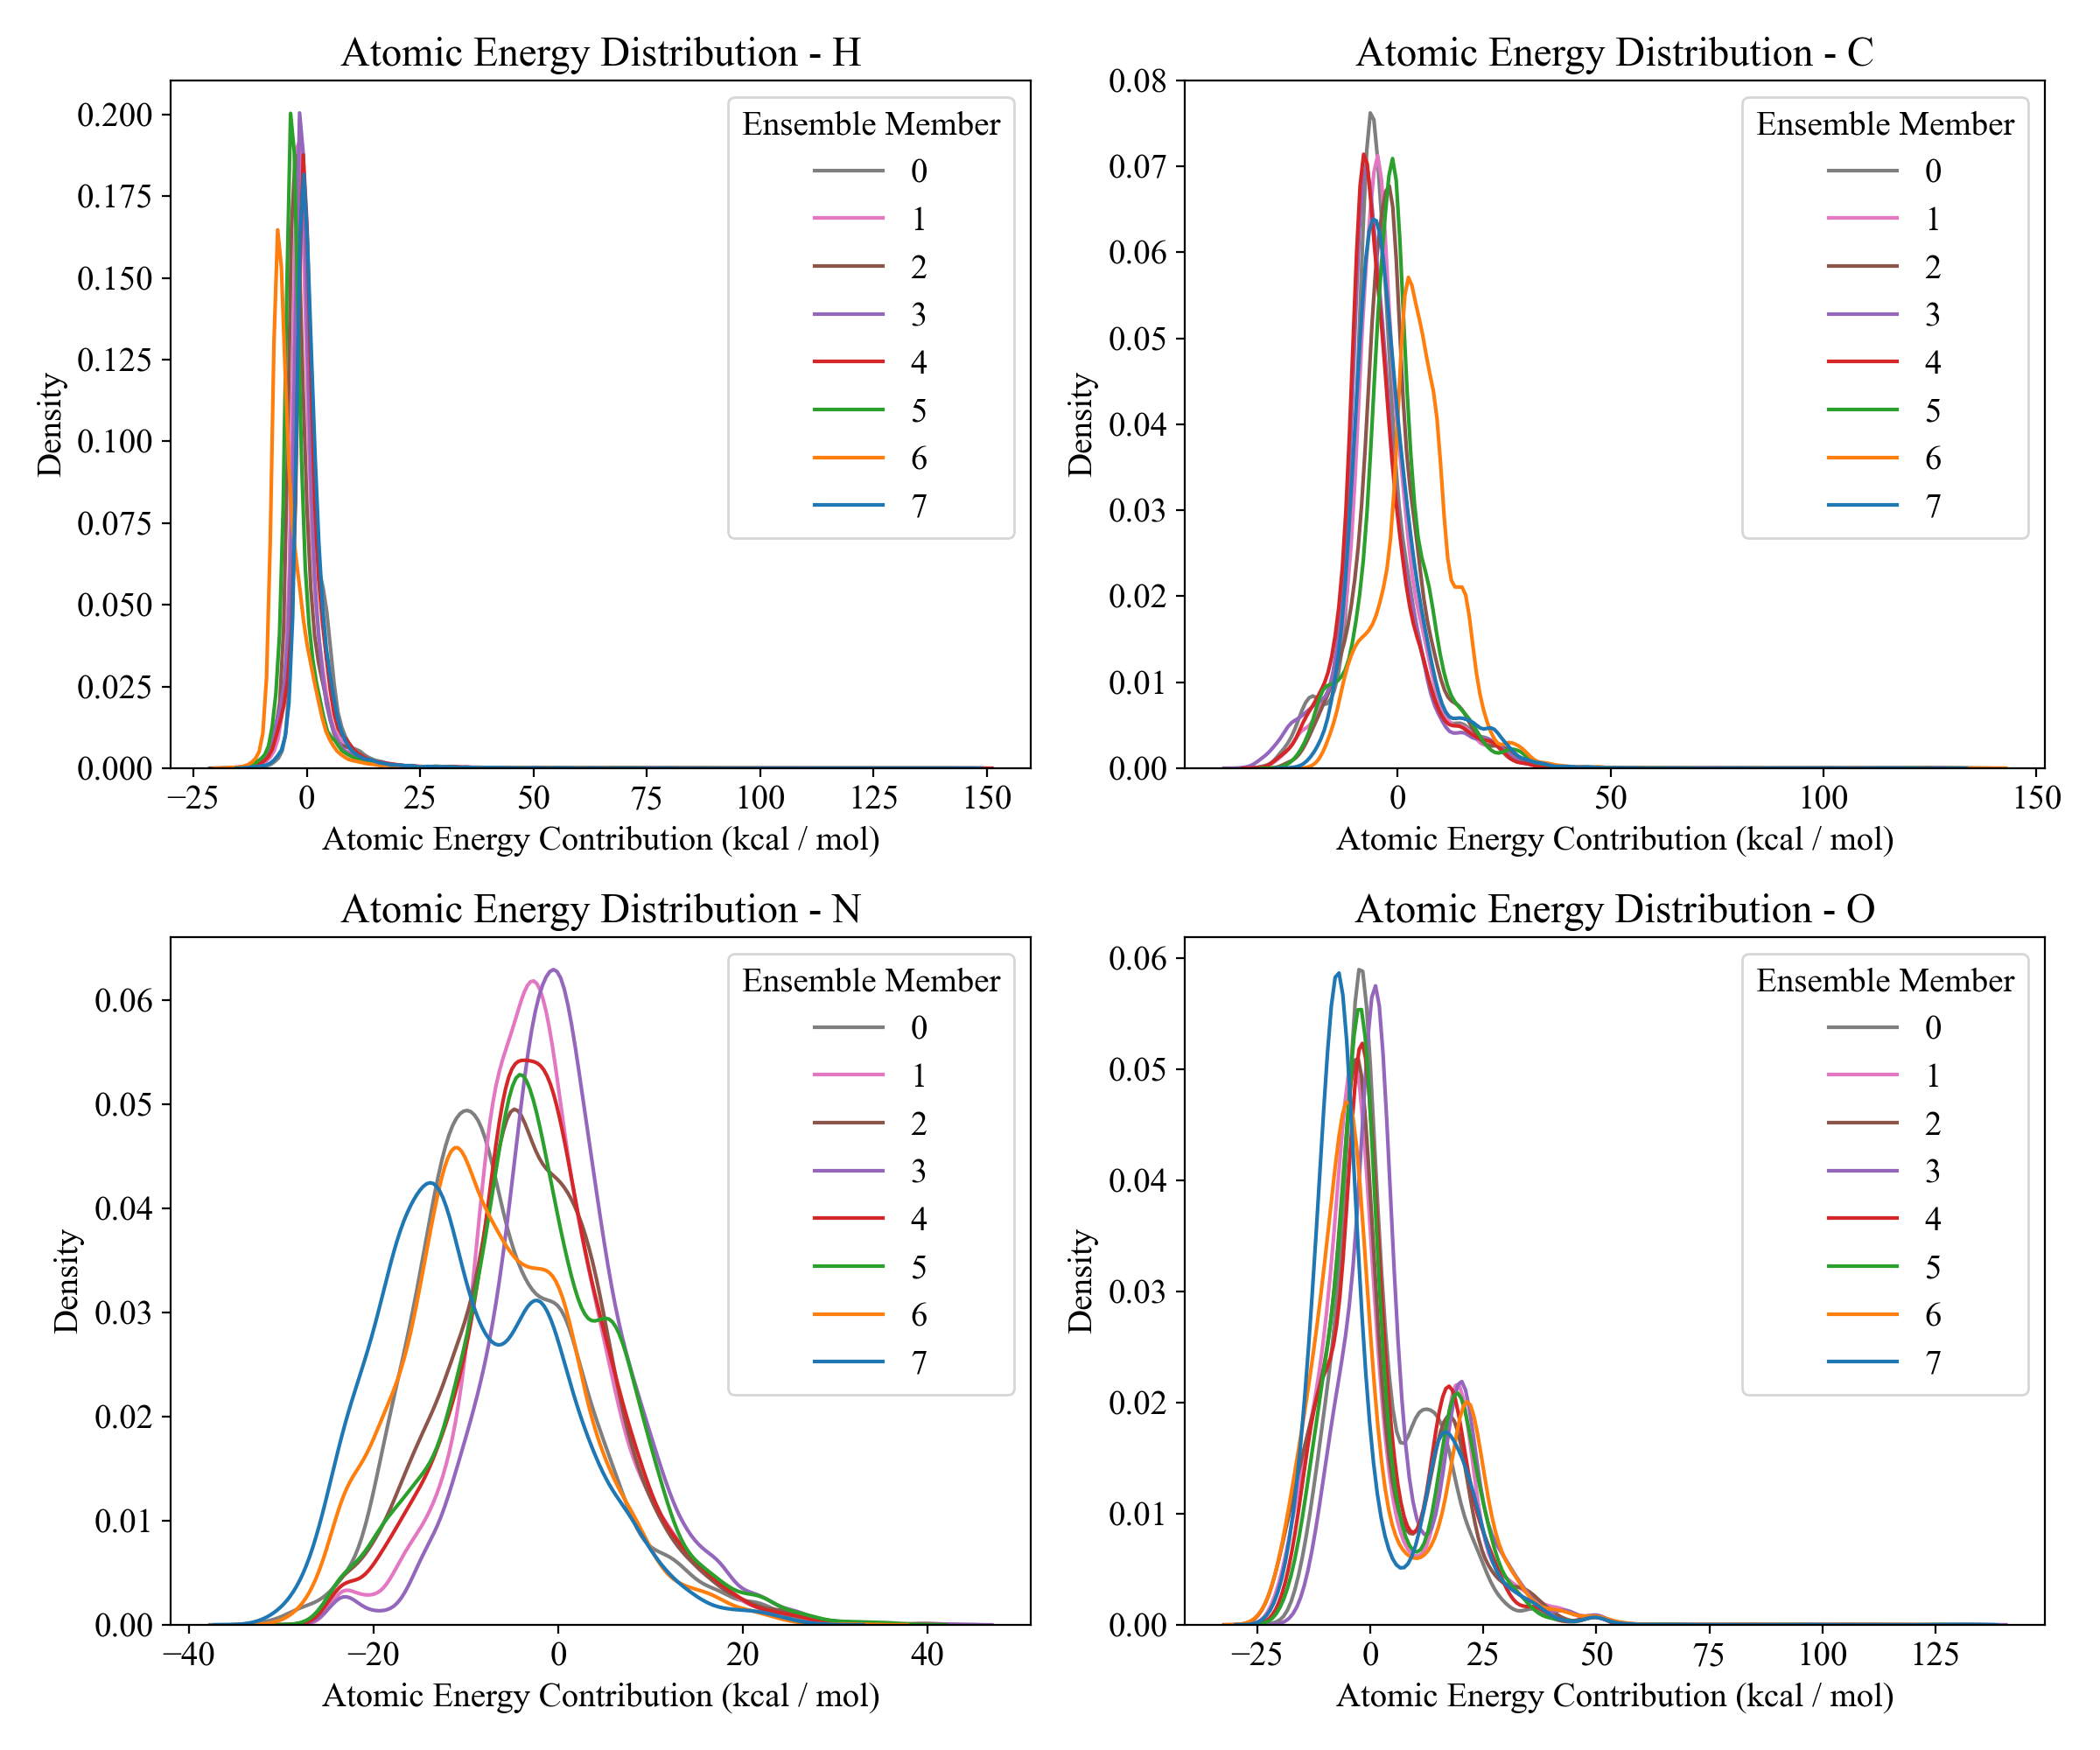
\includegraphics[width=1\linewidth]{Images/2x_outputs/2x_1x-first_ae-per-model.png}
    \caption{Think about remaking this with a consistent x-scale for all figures.}
    \label{fig:2x_ae_per_model}
\end{figure}

\authorRemark{You'll need to write something in between these to have the text spaced out properly.}

\begin{figure}[!ht]
    \centering
    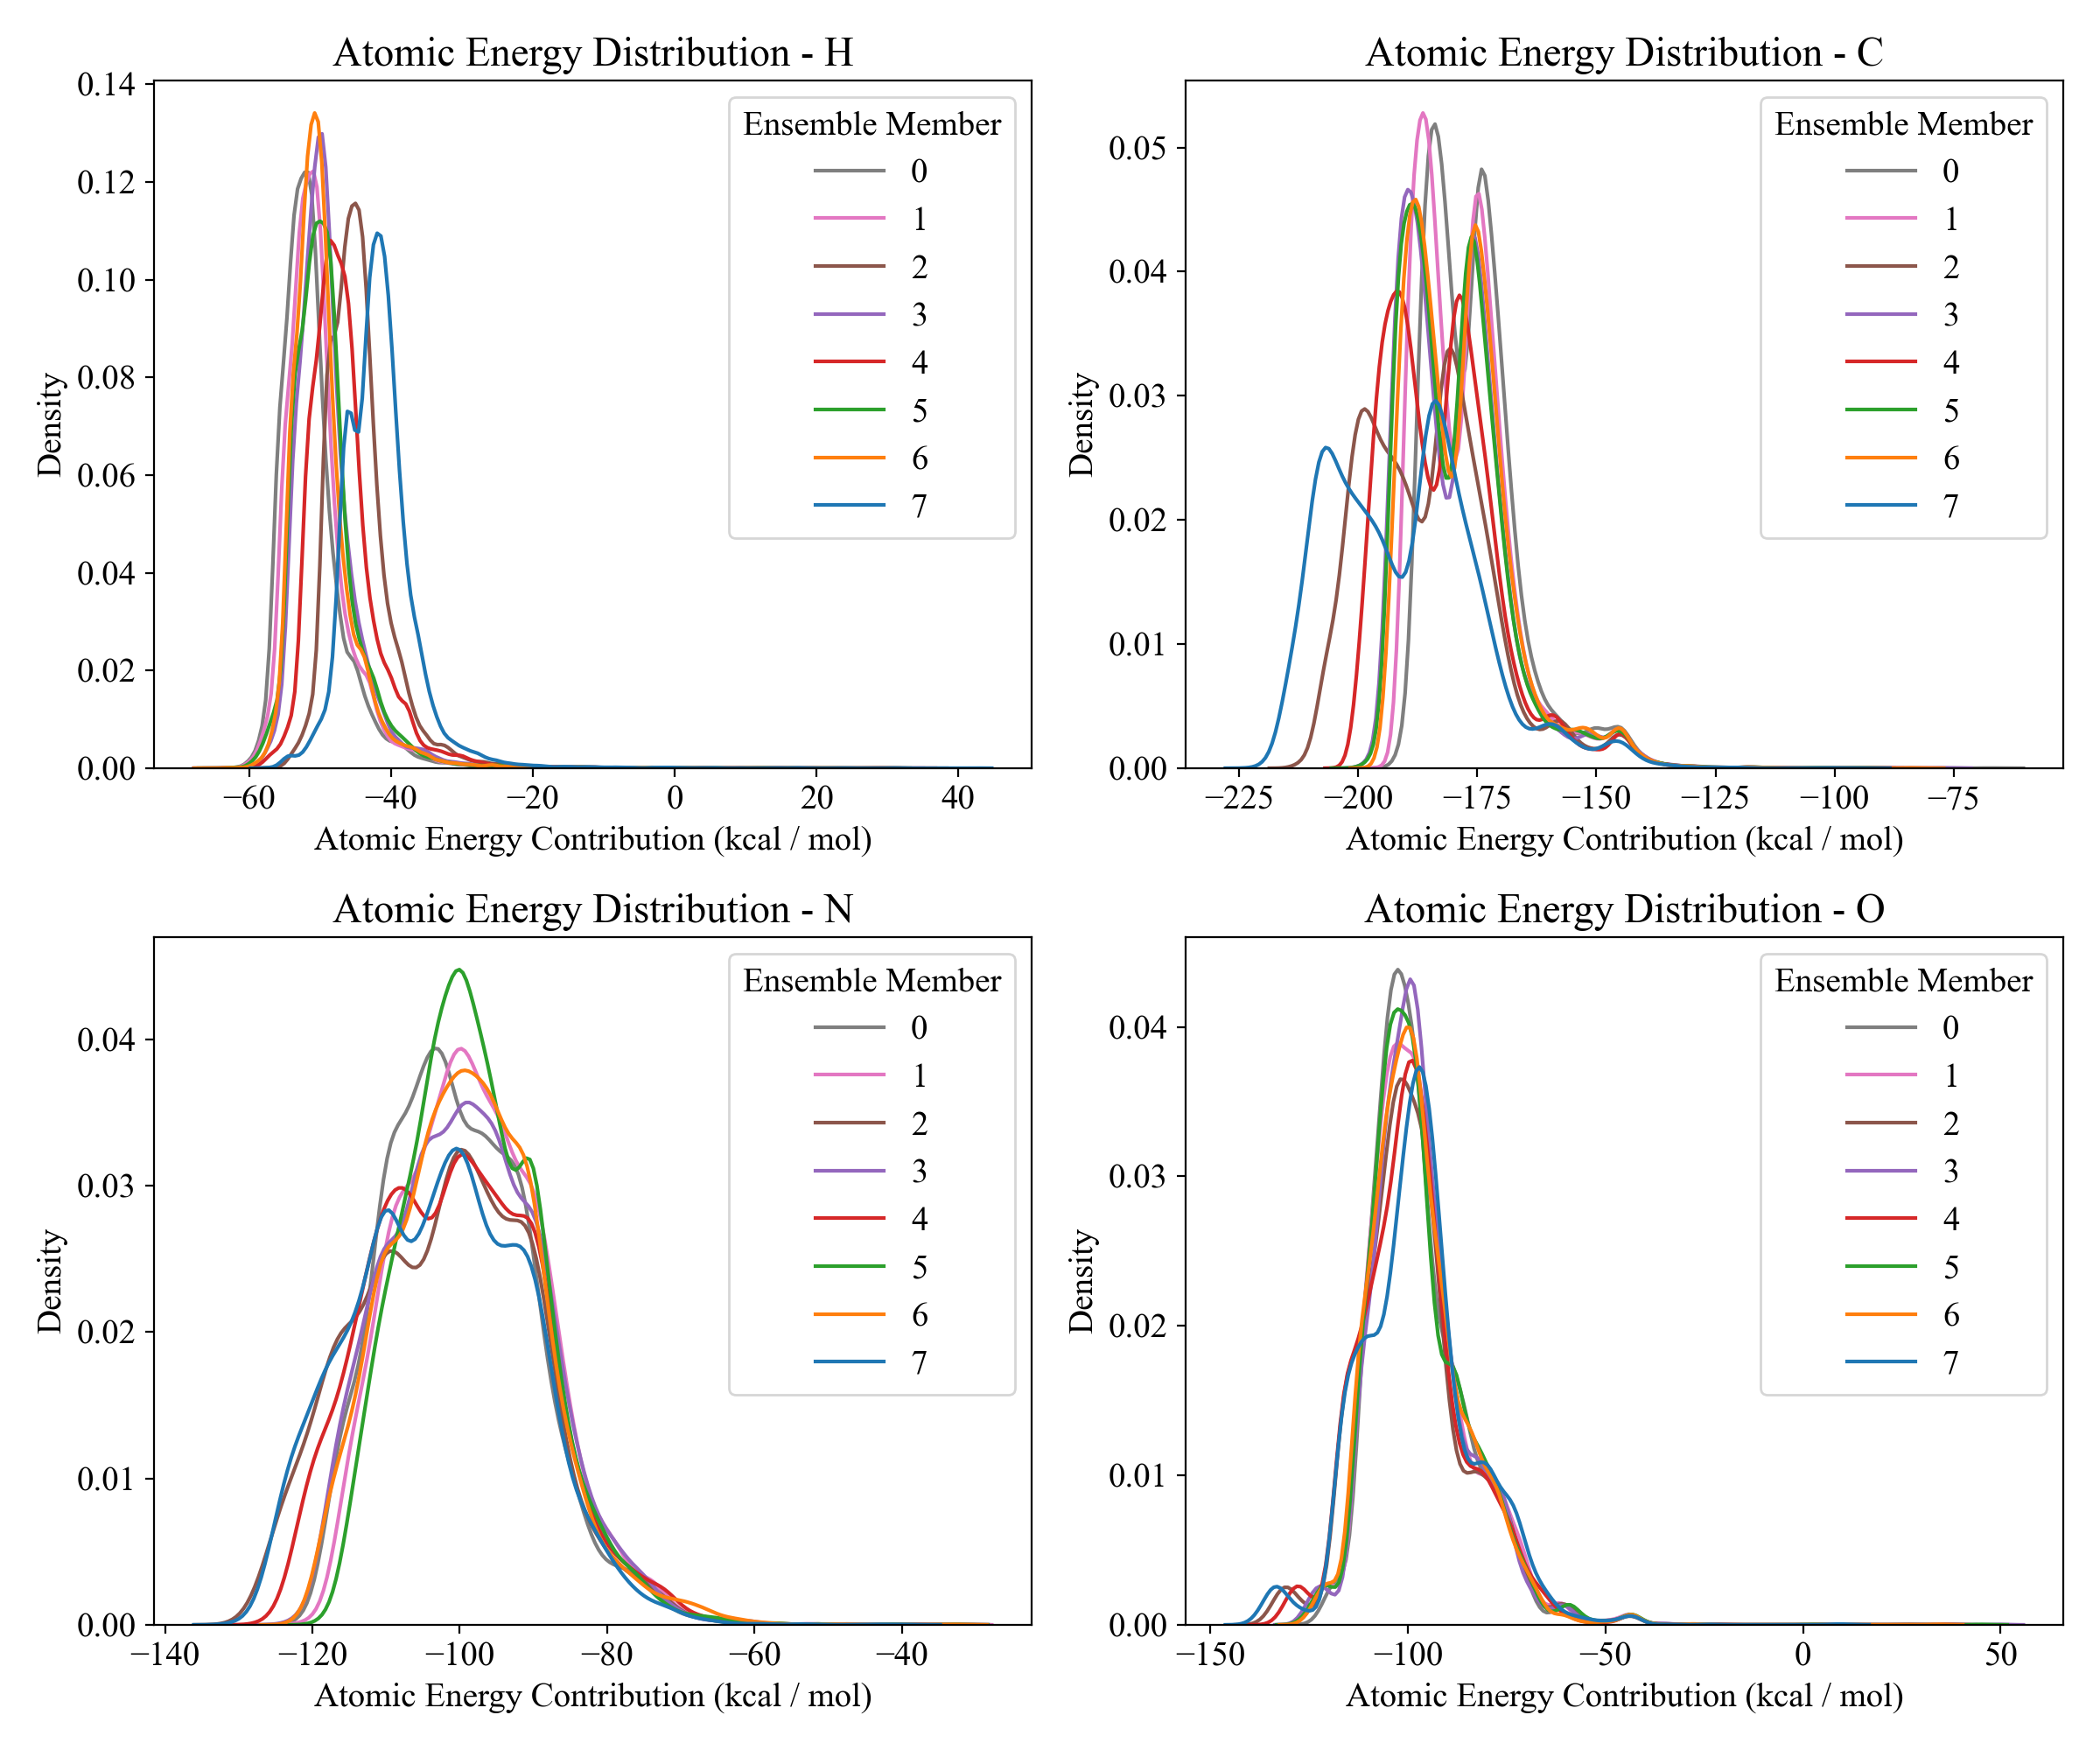
\includegraphics[width=1\linewidth]{Images/2xr_outputs/2xr_1x-first_ae-per-model.png}
    \caption{Think about remaking this with a consistent x-scale for all figures.}
    \label{fig:2xr_ae_per_model}
\end{figure}

Due to the parameters used in training (no biases, GSAEs rather than fitting to SAEs), 2xr is going to be the model used to discuss atomic trends after this.

\subsection{Uncertainty in ANI neural network potentials}
\label{subsec:ANI_uncertainty}

ANI potentials use an ensemble of 8 models.
Predictive uncertainty has been measured in published models using $\hat{rho}$; the value 0.23 kcal/mol was empirically chosen for sampling structures with high-error energy predictions via query by committee (QBC) in the active learning process \cite{ani-1x}.
The QBC, given in Eqn. \ref{eq:energy_qbc}, can be thought of as a binary classifier: 

\begin{equation}
\rho = \frac{\sigma_{E_{\text{Total}}}}{\sqrt{N_{\text{atoms}}}}
\label{eq:energy_qbc}
\end{equation}

\begin{figure}[!hb]
    \centering
    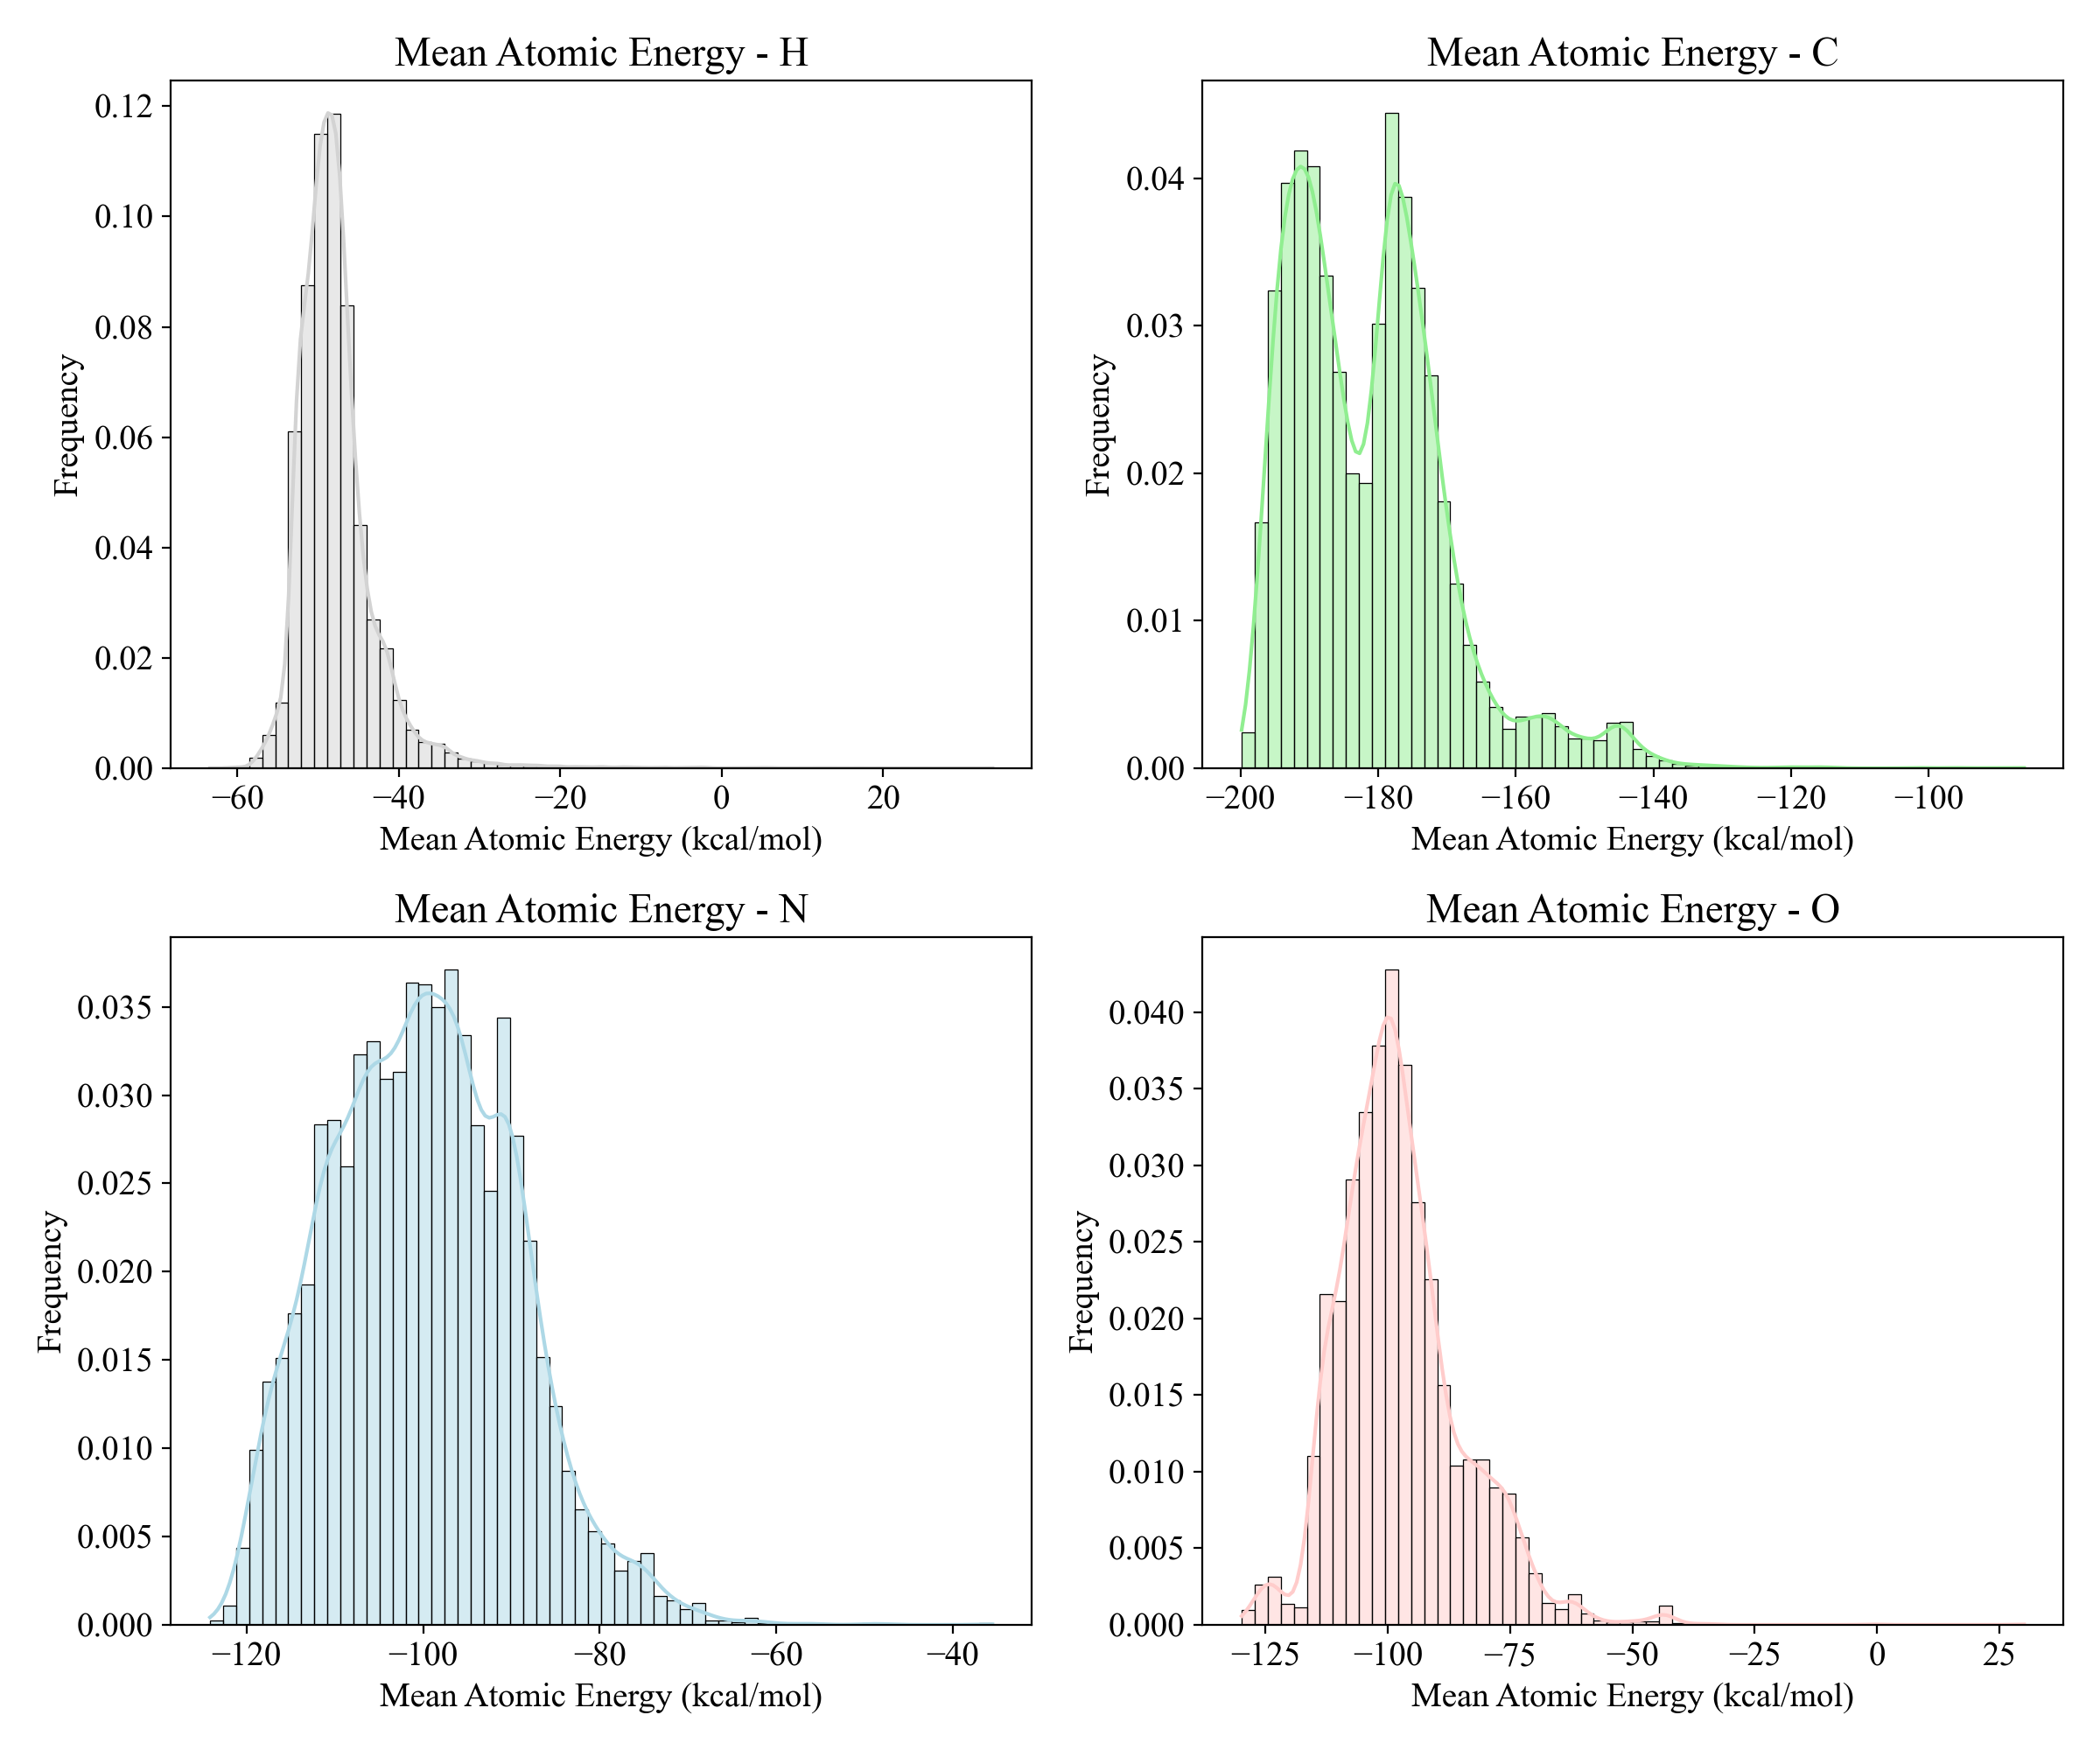
\includegraphics[width=1\linewidth]{Images/2xr_outputs/2xr_1x-first_mean-ae-per-atomtype.png}
    \caption{Caption}
    \label{fig:2xr_1x-first_mean-ae-per-atomtype}
\end{figure}

\subsection{Exploration of the flaws in predicting total energy as a sum of atomic energies}
\label{subsec:flaws_in_atomic_energies}

\authorRemark{MAKE PLOTS OF JUST CARBON STDEV, PLOT LINE ON TOTAL ENERGY STDEV GRAPH}

\begin{equation}
    \label{eq:covariance}
    \text{cov}(x, y) = \mathbb{E}[(x - \mathbb{E}[x])(y - \mathbb{E}[y])]
\end{equation}

insert images of hydrogen / carbon / nitrogen / oxygen stdev histograms, 



\section{Drawback of atomic energy predictions}



\begin{multiFigure}
\label{fig:ch4}
    \addFigure{1}{Images/ch4_example/ch4_2xr_stdev-ae.png}
    \addFigure{0.29}{Images/CH4.png}
    \addFigure{0.71}{Images/ch4_example/ch4_2xr_total-e-qbc.png}
\captionof{figure}[CH\textsubscript{4} atomic energy distribution]{CH4 atomic energy contributions, the red line signifies the ...}
\end{multiFigure}


% Tables suck, but this helped me align columns and headers separately:
\begin{table}[!hb]
\centering
\caption{
Atomic energy contributions by atom type in a geometry-optimized molecule of CH\textsubscript{4}, with four equivalent hydrogen atoms. 
Additionally, the sum over all atoms, and that sum after passing through the TorchANI EnergyShifter. 
Values obtained from an ensemble of ANI models (ANI2xr); the last column shows the standard deviation of predictions across the ensemble. 
All values are in kcal/mol.
}\label{tbl:ch4_AEs}
    \begin{tabularx}{\textwidth}{%
    >{\raggedleft\arraybackslash}r  % Numeric
    >{\raggedleft\arraybackslash}r  % Numeric
    >{\raggedleft\arraybackslash}r  % Numeric
    >{\raggedleft\arraybackslash}r  % Numeric
    >{\raggedleft\arraybackslash}r  % Numeric
    }  
Model & Carbon & Hydrogen  & Sum of atomic energies & Molecular energy \\
\hline
Mean prediction & -199.0069 & -55.1013 & -419.4123 & -25413.8125 \\
1 & -219.4329 &  -50.0170 &  -419.5012 &  -25413.9043 \\
2 & -194.7117 &  -56.1991 &  -419.5081 &  -25413.9102 \\
3 & -192.8823 &  -56.6466 &  -419.4689 &  -25413.8691 \\
4 & -201.5683 &  -54.4451 &  -419.3490 &  -25413.7500 \\
5 & -196.5227 &  -55.7060 &  -419.3471 &  -25413.7500 \\
6 & -212.9323 &  -51.5945 &  -419.3103 &  -25413.7109 \\
7 & -186.5623 &  -58.2018 &  -419.3694 &  -25413.7715 \\
8 & -187.4427 &  -58.0003 &  -419.4441 &  -25413.8457 \\
Standard deviation &  11.7621 &  2.9412 &  0.0775 &  0.0775 \\
\hline
\end{tabularx}
\end{table}



\section{Need for a practical, physical quantity to estimate uncertainty}

Looking for a correlation between the energy error and the predictive uncertainty of a given \textbf{atomic} quantity.

The ANI models excel at predicting molecular energies, but have also been trained to predict other properties, most notably forces, which are computed as a the second derivative of the potential energy surface. 

\begin{equation}
    Give\ the\ force\ loss\ here
\end{equation}


